\documentclass{article}
\usepackage{color}
\usepackage{amsmath}
\usepackage{graphicx}
\usepackage{geometry}
\usepackage{xcolor}
\usepackage{amssymb}
\geometry{letterpaper, total={170mm,257mm}, left=20mm, top=20mm}
\graphicspath{ {./images/} }
\newtheorem{theorem}{Theorem}[section]
\newcommand{\Lim}[1]{\raisebox{0.5ex}{\scalebox{0.8}{$\displaystyle \lim_{#1}\;$}}}
\newcommand{\p}{\partial}
\newcommand{\dg}{^{\circ}}
\newcommand{\tri}{\vec{\bigtriangledown}}
\newcommand{\mat}[4]{\begin{bmatrix} #1 & #2 \\ #3 & #4 \end{bmatrix}}
\newcommand{\mathree}[9]{\begin{bmatrix} #1 & #2 & #3 \\ #4 & #5 & #6 \\ #7 & #8 & #9 \end{bmatrix}}
\newcommand{\der}[2]{\frac{d #1}{d #2}}
\newcommand{\pat}[2]{\frac{\partial #1}{\partial #2}}
\newcommand{\Int}[2]{\int_{#1}^{#2}}
\newcommand{\Sum}[2]{\sum_{#1}^{#2}}
\newcommand{\eval}[2]{\bigg|_{#1}^{#2}}
\newenvironment{ind}[1]
 {\begin{list}{}
         {\setlength{\leftmargin}{#1}}
         \item[]
 }
 {\end{list}}

\title{Vector Calculus}
\author{Justin Bornais}
\date{May 11, 2023}

\begin{document}
\maketitle

\section{Construction of a Line}
\subparagraph{}
The equation of a line is $y=mx+b$, where $y$ is the dependent variable and $x$ is the dependent variable. Now, the equation of a line passing through ($x_0,y_0,z_0$) (or $\vec{r_0}$) and is parallel to the vector $\vec{v}$ is $\vec{r}=\vec{r_0}+t\vec{v}, t\in R$
\section{Planes}
\subparagraph{}
The equation of the plane is $ax+by+cz=d$ where $\vec{n}=<a,b,c>$ is the normal vector of the plane.
\subsection{Cylinders}
A \textbf{cylinder} is a surface that consists of all lines parallel to a line and passing through $a$.
\paragraph[Examples]{Examples: Identify and sketch the surface}
\subparagraph{1. $x^2+y^2=4\rightarrow \text{a circle in 2 dimensions} $}
$x^2+y^2=4$ is a cylinder in 3 dimensions (a surface where one variable is missing is a cylinder, the missing variable is the axis).
\subparagraph{2. $y^2+z^2=9$} A cyliinder with x-axis as the axis.
\subparagraph{3. $z=x^2$} A cylinder with y-axis as the axis.

\section{Quadrics}
A quadric in two dimensions is:
\begin{enumerate}
    \item A parabola $y=x^2$ or $x=y^2$
    \item An ellipse: $\frac{x^2}{a^2}+\frac{y^2}{b^2}=1$
    \item A hyperbola: $\frac{x^2}{a^2}-{y^2}{b^2}=1$
\end{enumerate}
A trace is the curve of the intersection of the surface with the coordinate plane $\rightarrow$ 3 traces.
\newpage
\subsection{Quadric Surface}
$Ax^2+By^2+Cz^2+Dxy+Exz+Fzy+Gx+Hy+Iz+J=0$
\newline In this course, we need to know 6 quadric surfaces.\newline
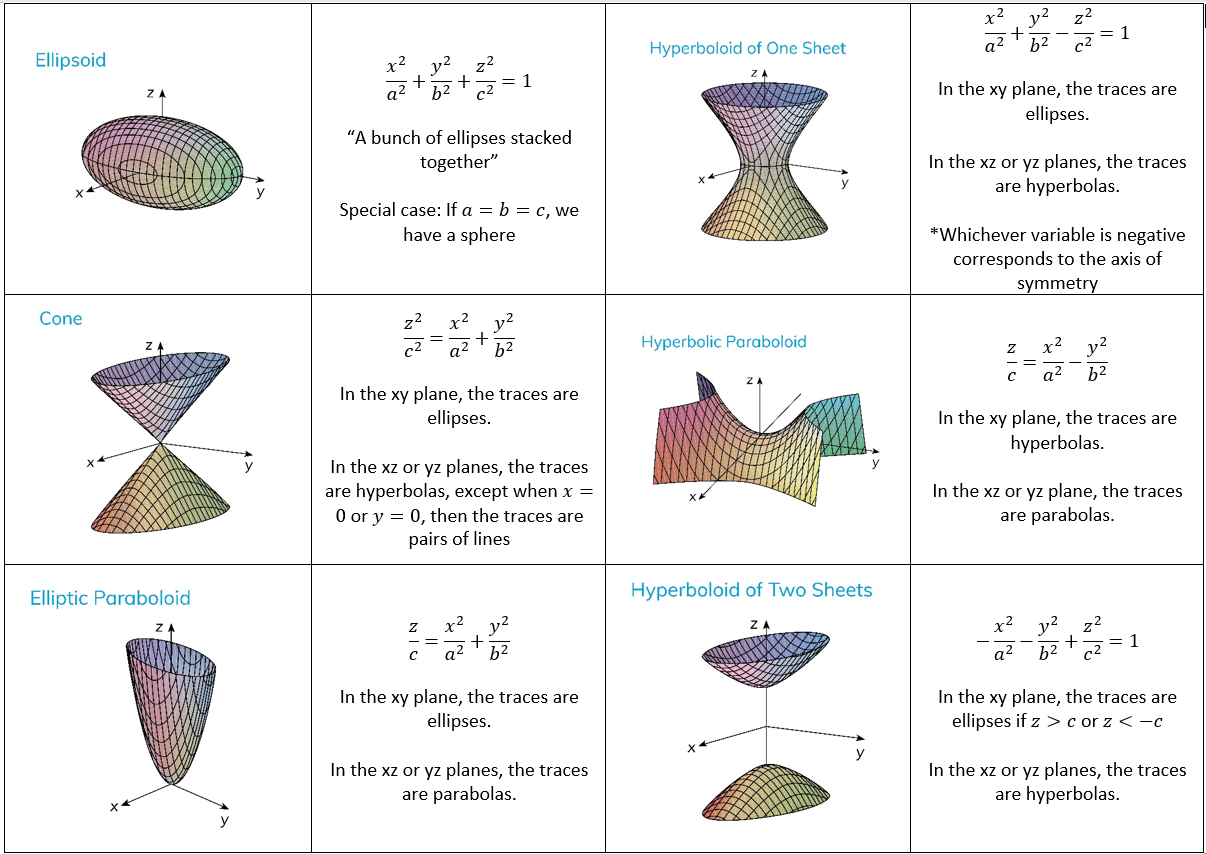
\includegraphics[width=\textwidth]{quadric_surfaces.png}

\paragraph{} We can actually know some patterns for the rest of the quadric surfaces:
\begin{itemize}
    \item \textbf{Ellipsoid} $\Rightarrow \frac{x^2}{a^2}+\frac{y^2}{b^2}+\frac{z^2}{c^2}=1$
    \item \textbf{Hyperboloid of One Sheet} $\Rightarrow \frac{x^2}{a^2}+\frac{y^2}{b^2}-\frac{z^2}{c^2}=1$
    \item \textbf{Hyperboloid of Two Sheets} $\Rightarrow -\frac{x^2}{a^2}-\frac{y^2}{b^2}+\frac{z^2}{c^2}=1$
    \item \textbf{Cone} $\Rightarrow \frac{z^2}{c^2}=\frac{x^2}{a^2}+\frac{y^2}{b^2}$
    \item \textbf{Elliptic Paraboloid} $\Rightarrow  \frac{z}{c}=\frac{x^2}{a^2}+\frac{y^2}{b^2}$
    \item \textbf{Hyperbolic Paraboloid} $\Rightarrow  \frac{z}{c}=\frac{x^2}{a^2}-\frac{y^2}{b^2}$
\end{itemize}
Notice the patterns with the equations?
\newpage
\subsubsection{Elliptic Paraboloids}
The equation of an elliptic paraboloid is $\frac{z}{c}=\frac{x^2}{a^2}+\frac{y^2}{b^2}$ where $z$ is the axis, $xy$ traces are ellipses ($x=0$) and both $\frac{x^2}{a^2}$ and $\frac{y^2}{b^2}$ have the same signs.
\newline \indent 2 traces is a parabola, 1 trace is an ellipse.
\newline\newline Effectively, the variable with a power of $1$ is the axis.
\subparagraph{$z=0$}$\Rightarrow 0=\frac{x^2}{a^2}+\frac{y^2}{b^2} \Rightarrow x=0,y=0,z=0$
\subparagraph{$z=k$}$\Rightarrow \frac{k}{c}=\frac{x^2}{a^2}+\frac{y^2}{b^2} \Rightarrow$ ellipses for $k>0$

\subsubsection{Hyperboloid of One Sheet}
The variable with the negative sign is the axis. The \textbf{xy-trace} is where $z=0$. The \textbf{xz-trace} and \textbf{yz-trace} is a hyperbola.

\subsubsection{Hyperboloid of Two Sheets}
The variable with the positive sign is the axis. The \textbf{xy-trace} is an ellipses if $\lvert z \rvert > \lvert c \rvert $

\subsubsection{Cone}
The variable with the negative sign is the axis. Two traces are hyperbolas, one trace is an ellipse for $k\ne 0$.

\subsubsection[Exampls]{Examples: Identify and sketch the surfaces}
\paragraph{1. $x^2+4y^2+z^2=4$} $\Rightarrow \frac{x^2}{4}+\frac{y^2}{4}+\frac{z^2}{4}=1$
\paragraph{3. $z^2=x^2+4y^2+64$} $\Rightarrow -x^2-4y^2+z^2=64$
$\Rightarrow -\frac{x^2}{64}-\frac{y^2}{16}+\frac{z^2}{64}=1$ (hyperboloid on 2 sheets, axis is z-axis with $c=8$)

\newpage
\section{Vector Functions}
These are chapters 13.1 and 13.2 from last class.

A vector function is $\vec{r}(t)=<f(t),g(t),h(t)>$ such that $f(t)=x$, $g(t)=y$ and $h(t)=z$.
\begin{itemize}
    \item For 2 dimensions: $\vec{r}(t)=<f(t),g(t)>$
    \item $\vec{r}\,'(t)=<f'(t),g'(t)>$ or $\vec{r}\,'(t)=<f'(t),g'(t),h'(t)>$
\end{itemize}

\subsection{Arc Length}
The equation for length is $|\vec{r}\,'(t)|=\sqrt{(f'(t))^2+(g'(t))^2}$ for 2 dimensions,
or $|\vec{r}\,'(t)|=\sqrt{(f'(t))^2+(g'(t))^2+(h'(t))^2}$ for 3 dimensions.

Now, the formula is effectively $\sqrt{(\delta x)^2 + (\delta y)^2}$, where $x=f(t)$ and $\delta x=f'(t)dt$ and similarly for $y$.
\\Thus the formula is $\sqrt{(f'(t)dt)^2+(g'(t)dt)^2}=\sqrt{(f'(t))^2+(g'(t))^2(dt)^2}=\sqrt{(f'(t))^2+(g'(t))^2}dt$
\\\\\textbf{Arc Length is: } $L=\int_{a}^{b} \sqrt{(f'(t))^2+(g'(t))^2}dt$
\\Thus, the arc length of a curvee $\vec{r}(t)$ for $a\leq t\leq b$ is $\int_{a}^{b} |\vec{r}\,'(t)|dt$

\subsection{Example 1}
Find the length of the curve $\vec{r}(t)=<2\sin^3t,2cos^3t>, 0\leq t\leq \frac{\pi}{4}$
\\\\\textbf{Solution:} $\vec{r} '(t)=<2(3\sin^2t)(\cos t), 2(3\cos^2t)(-\sin t)>$
\\$|\vec{r}\,'(t)|=\sqrt{(6sin^2t \cos t)^2+(-6\cos^2t \sin t)^2}$
\\$=\sqrt{36\sin^4t \cos^2t+36\cos^4t\sin^2t}$
\\$=\sqrt{36\sin^2t\cos^2t(\sin^2t+\cos^2t)}$
\\$=\sqrt(36\sin^2t\cos^2t(1))$
\\$=6\sin t\cos t$
\\\\The arc length $L=\int_{a}^{b} |\vec{r}\,'(t)|dt=\int_{0}^{\frac{\pi}{4}} 6\sin t\cos tdt$
\\Let $u=\sin t$ so $du=\cos tdt$
\\\\Then we have $L=\int_{0}^{\frac{\pi}{4}} 6udu=\frac{6u^2}{2}=3u^2$
\\$=3\sin^2t |_{t=0}^{\frac{\pi}{4}}=3\sin^2\frac{\pi}{4}-3\sin^20=3(\frac{1}{2})=\frac{3}{2}$

\subsection{Example 2}
Find the length of the curve $\vec{r}(t)=<t^2,2t,\ln t>, 1\leq t\leq e$
\\\\\textbf{Solution:} $\vec{r}\,'(t)=<2t,2,\frac{1}{t}>$
\\$|\vec{r}\,'(t)|=\sqrt{4t^2+4+\frac{1}{t^2}}=\sqrt{\frac{4t^4+4t^2+1}{t^2}}=\frac{\sqrt{(2t^2+1)^2}}{\sqrt{t^2}}=\frac{2t^2+1}{t}$
\\$L=\int_{a}^{b} |\vec{r}\,'(t)|dt=\int_{1}^{e} \frac{2t^2+1}{t}dt=\int_{1}^{e} \left(\frac{2t^2}{t}+\frac{1}{t}\right)dt$
\\$L=\int_{1}^{e} \left(2t+\frac{1}{t}\right)dt=t^2+\ln |t|\,\,|_{1}^{e}$
\\$L=e^2+\ln |e|-1^2-\ln 1=e^2$

\newpage
\subsection{Curvature}
In the last class, the unit tangent vector $\vec{T}(t)=\frac{\vec{r}\,'(t)}{|\vec{r}\,'(t)|}$.
Curvature is the magnitude of the rate of change of the unit tangent vector w.r.t. the arc length.
\\\\\textbf{Arc Length Function} $S=\int_{a}^{t}\left|\vec{r}\,'(u) \right|du$
\\\textbf{Curvature Function} $K=\left|\frac{d\vec{T}}{ds}\right|$
\begin{itemize}
    \item Note: $\frac{d\vec{T}}{dt}=\frac{d\vec{T}}{ds}\frac{ds}{dt} \rightarrow$ chain rule.
    \\ $\frac{d\vec{T}}{dt}=\frac{d\vec{T}}{ds}|\vec{r}\,'(t)|\Rightarrow \left|\frac{d\vec{T}}{ds}\right|=\frac{\left|\frac{d\vec{T}}{dt}\right|}{|\vec{r}\,'(t)|}=\frac{|\vec{T}\,'(t)|}{|\vec{r}\,'(t)|}$
    \item Thus $K=\frac{|\vec{T}\,'(t)|}{|\vec{r}\,'(t)|}$
    \item Another formula for $K=\frac{|\vec{r}\,'(t)\times\vec{r}\,''(t)|}{|\vec{r}\,'(t)|^3}$
\end{itemize}

\subsection{Example 1}
Find the curvature of the following curve: $\vec{r}(t)=<5\sin t,3t, 5\cos t>$
\\\\\textbf{Solution:} $\vec{r}\,'(t)=<5\cos t,3,-5\sin t>$, $|\vec{r}\,'(t)=\sqrt{25\cos^2t+9+25\sin^2t}=\sqrt{25(\cos^2t+\sin^2t)+9}=\sqrt{34}$
\\$\vec{T}(t)=\frac{\vec{r}\,'(t)}{|\vec{r}\,'(t)}=\frac{<5\cos t,3,-5\sin t>}{\sqrt{34}}$
\\$\vec{T}\,'(t)=\frac{1}{\sqrt{34}}<-5\sin t,0,-5\cos t>$
\\$\left|\vec{T}\,'(t)\right|=\sqrt{\frac{1}{34}\left(25\sin^2t+25\cos^2t\right)}=\sqrt{\frac{25}{34}}=\frac{\frac{5}{\sqrt{34}}}{\sqrt{34}}$ (divide by $\sqrt{34}$ one more time since we're trying to find $K$)

\subsection{Example 2}
Find the curvature of the following curve: $\vec{r}\,'(t)=<t,t,1+t^2>$
\\\\\textbf{Solution:} $\vec{r}\,'(t)=<1,1,2t>$, $|\vec{r}\,'(t)|=\sqrt{1^2+1^2+4t^2}=\sqrt{2+4t^2}
\\\vec{T}\,'(t)=\frac{\vec{r}\,'(t)}{|\vec{r}\,'(t)}=\frac{<1,1,2t>}{\sqrt{2+4t^2}}=\left<\frac{1}{\sqrt{2+4t^2}},\frac{1}{\sqrt{2+4t^2}},\frac{2t}{\sqrt{2+4t^2}} \right>$
\\$\vec{T}\,'(t)=...$ (hard to calculate)
\\\textbf{Instead, another formula for K:} $K=\frac{|\vec{r}\,'(t)\times\vec{r}\,''(t)|}{|\vec{r}\,'(t)|^3}$
\\$\vec{r}\,''(t)=<0,0,2>$
\\$\vec{r}\,'(t)\times\vec{r}\,''(t)=\begin{bmatrix}
    \hat{i} & \hat{j} & \hat{k} & \\
    1 & 1 & 2t \\
    0 & 0 & 2
\end{bmatrix}=\hat{i}(2-0)-\hat{j}(2-0)+\hat{k}(0-0)=2\hat{i}-2\hat{j}+0\hat{k}\;or\;<2,-2,0>$ (remember cross product in MATH1250)
\\$K=\frac{|\vec{r}\,'(t)\times\vec{r}\,''(t)|}{|\vec{r}^3|}=\frac{\sqrt{8}}{\left(\sqrt{2+4t^2}\right)^3}$
\newpage

\section{(13.4) Motion in Space}
We learned that $\vec{r}(t)=<f(t),g(t),h(t)>$ where $f(t)=x$, $g(t)=y$ and $h(t)=z$.
\begin{itemize}
    \item If the position vector/function of an object is $\vec{r}(t)=<f(t),g(t),h(t)>$ then the velocity of the object is $\vec{v}(t)=\vec{r}\,'(t)$ and it will be in the direction of the tangent vector $\vec{r}\,'(t)$.
    \item The speed is $\left|\vec{v}(t)\right|=\left|\vec{r}\,'(t)\right|$
    \item The acceleration of the object is $\vec{a}(t)=\vec{v}\,'(t)=\vec{r}\,''(t)$
\end{itemize}

\subsubsection{Example 1}
Find the velocity, acceleration and speed of a particle with position vector (function) $\vec{r}(t)=<e^t,t^4,e^{-t}>$

\paragraph{Solution} $\vec{v}(t)=\vec{r}\,'(t)=<e^t,4t^3,-e^{-t}>\;\rightarrow\text{velocity}$
\\Acceleration is $\vec{a}(t)=\vec{v}\,'(t)=<e^t,12t^2,e^{-t}>$
\\Speed is $|\vec{v}(t)|=\sqrt{\left(e^t\right)^2+\left(4t^3\right)^2+\left(e^{-t}\right)}=\sqrt{e^{2t}+16t^6+e^{-2t}}$


\subsubsection{Example 2}
Find the velocity, acceleration and speed of a particle with position vector $\vec{r}(t)=<e^t,t^4,e^{-t}>$ at $t=0$.

\paragraph{Solution} From example 1, $\vec{v}(t)=<e^t,4t^3,-e^{-t}>$
\\At $t=0$, the velocity is $\vec{v}(0)=<e^0,4(0)^3,-e^{-0}>=<1,0,-1>$
\\The speed at $t=0$ is $\sqrt{1^2+0^2+(-1)^2}=\sqrt{2}$
\\$\vec{a}(t)=<e^t,12t^2,e^{-t}>$
\\At $t=0$, $\vec{a}(0)=<e^0,12(0)^2,e^{-0}>=<1,0,1>$

\subsubsection{Example 3}
Given the acceleration vector $\vec{a}(t)=<2t,1,t^2>$ amd the initial velocity is $\vec{v}(0)=<0,1,1>$
and the initial position vector is $\vec{r}(0)=<2,0,-1>$, find the velocity and position vectors of the particle.

\paragraph{Solution}
The velocity is $\vec{v}(t)=\int \vec{a}(t)dt=\int <2t,1,t^2>dt
\\=<\frac{2t^2}{2}+C_1,t+C_2,\frac{t^3}{3}+C_3>\;\text{or }<t^2,t,\frac{t^3}{3}>+<C_1,C_2,C_3> (\vec{C})$
\\$\vec{v}(0)=<0,1,1>\Rightarrow<0,1,1>=<0+C_1,0+C_2,0+C_3>\Rightarrow C_1=0, C_2=1, C_3=1$
\\Thus the velocity is $\vec{v}(t)=<t^2,t+1,\frac{t^3}{3}+1>$
\\\\The position vector is $\vec{r}(t)=\int \vec{v}(t)dt=\int<t^2,t+1,\frac{t^3}{3}+1>dt$
\\$\vec{r}(t)=<\frac{t^3}{3}+d_1,\frac{t^2}{2}+t+d_2,\frac{t^4}{12}+t+d_3>$
\\$\vec{r}(0)=<2,0,-1>\Rightarrow<2,0,-1>=<0+d_1,0+d_2,0+d_3>\Rightarrow d_1=2,d_2=0,d_3=-1$
\\So $\vec{r}(t)=<\frac{t^3}{3}+2,\frac{t^2}{2}+t,\frac{t^4}{12}+t-1>$

\section{Functions of Several Variables (or Multivariable Functions)}
\textbf{Multivariable Functions} are functions with at least 2 independent variables.
In \textbf{chapters 14 and 15}, we cover domains, limits, continuity, derivatives
and applications, integration and applications. \begin{itemize}
    \item One prominent example is the volume functions $V=xyz$ and $V=\pi r^2h$
\end{itemize}

\subsection{Functions of 2 Variables}
$x$ and $y$ are independent variables, and the domain will be in $R^2$:
$D=\{(x,y)\;|\;\text{properties}\}$
\\A function in 2 variables, $z=f(x,y)$ is a rule that assigns to each $(x,y)\in D$ a unique value $z$ in $R$.
\begin{itemize}
    \itemsep 0em
    \item The domain $D$ is $R^2$ (inputs).
    \item The range is a subset of $R$ (outputs).
    \item $z=f(x,y)\rightarrow\;\text{explicit.}$
    \item $f(x,y,z)=0\rightarrow\;\text{implicit.}$
\end{itemize}

The vertical line test (VLT) can be used to check if a single-variable relation is a function.
This is similar for 2-variable functions, the VLT will instead draw lines parallel to the z-axis.
The relation will be a function if every vertical line crosses the surface of a function only once.

\subsubsection{Example 1}
Find the domain of $f(x,y)=\ln(x+y)$
\paragraph{Solution} We need $x+y>0\Rightarrow y>-x$
\\Thus the domain of $f=\{(x,y)\;|\;y>-x\}$

\subsubsection{Example 2}
Find the domain of $f(x,y)=\sqrt{1+x-y^2}$

\paragraph{Solution} We need $1+x-y^2\geq0\Rightarrow x\geq y^2-1$
\\Thus the domain of $f=\{(x,y)\;|\;x\geq y^2-1\}$

\subsection{Sketch the Domains}
Draw $x=y^2-1$\\
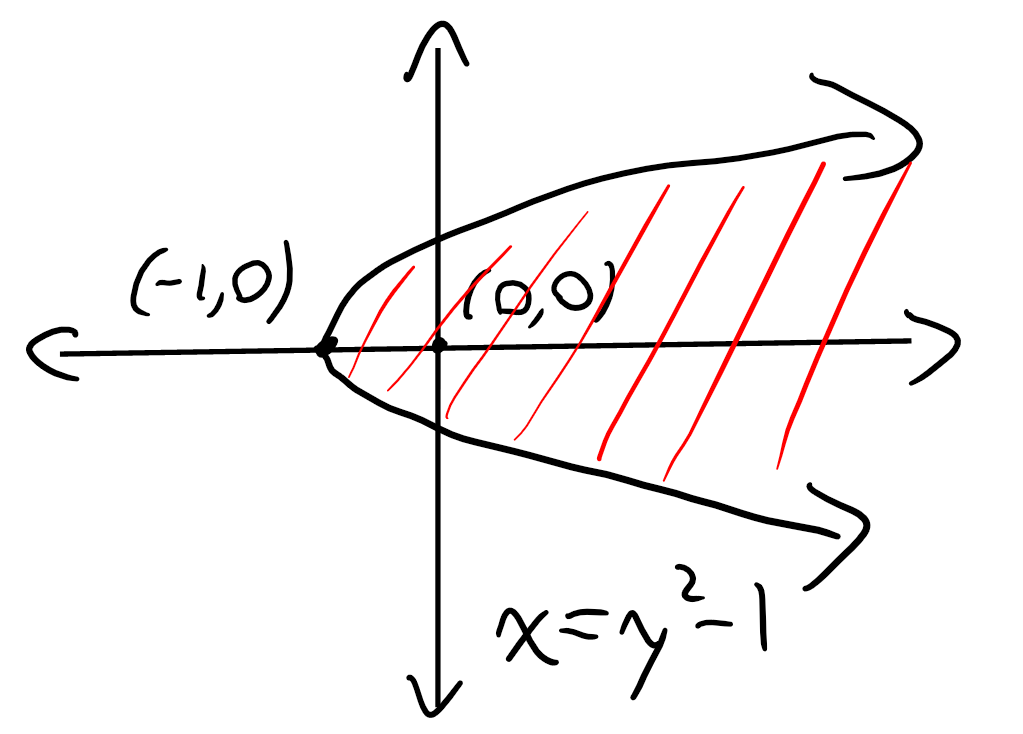
\includegraphics[width=200px]{sketch-domain.png}
\\Choose a test point, (0,0)
\\$x\geq y^2-1\Rightarrow0\geq0-1\Rightarrow0\geq-1\;\text{True}\Rightarrow \text{Shade the side that has (0,0)}$
\\Graphing the surface $z=f(x,y)$ will be in 3 dimensions.

\subsubsection{Example 1}
Sketch the graph of the following function: $f(x,y)=8-x-2y$

\paragraph{Solution} $z=8-x-2y\Rightarrow x+2y+z=8\Rightarrow\;\text{a plane}$
\\x-intercept: $y=0,z=0\Rightarrow x=8\Rightarrow(8,0,0)$
\\y-intercept: $x=0,z=0\Rightarrow 2y=8\Rightarrow y=4\Rightarrow(0,4,0)$
\\z-intercept: $x=0,y=0\Rightarrow z=8\Rightarrow(0,0,8)$

\subsubsection{Example 2}
Sketch the graph of the following function: $f(x,y)=\sqrt{2x^2+y^2}$

\paragraph{Solution} $z=\sqrt{2x^2+y^2}\Rightarrow z^2=2x^2+y^2\Rightarrow 2x^2+y^2-z^2=0\Rightarrow\;\text{a cone}$

\subsubsection{Example 3}
Sketch the graph of the following function: $f(x,y)=-\sqrt{2x^2+y^2}$

\newpage\subsection{(14.1) Functions}
In last class, we did functions of 2 variables, such as $z=f(x,y)$ where $(x,y)\in D$ where $D$ is the domain in $R^2$.
However, this idea can be extended to more than 2 variables. A 3-variable function would have $w=f(x,y,z)$ (explicit form) or $f(x,y,z,w)=0$ (implicit form).

\subsubsection{Example}
Find the domain of $f(x,y,z)=\frac{1}{\sqrt{16-x^2-y^2-z^2}}$ and sketch it.
\paragraph{Solution} For the domain, we need $16-x^2-y^2-z^2>0$.
\\$D=\{(x,y,z)\;|\;16-x^2-y^2-z^2>0\}$ (or $x^2+y^2+z^2<16$)
\\\\To sketch, draw $x^2+y^2+z^2=16$ (a sphere with a radius of $\sqrt{16}=4$). $(0,0,0)\Rightarrow 0+0+0<16\Rightarrow0<16$

\subsection{Limits and Continuity}
$\Lim{x\to a} f(x)=L$ if $f(x)\rightarrow L$ as $x\rightarrow a$ and the righthand/lefthand limits are equal to L.
\\$\Lim{(x,y)\to(a,b)} f(x,y)=L$ if $f(x,y)\rightarrow L$ as $(x,y)\rightarrow(a,b)$ along every possible path.
\\If two paths give different answers, then this proves the limit DNE. To find the limit, when it exists, we substitute $x=a$ and $y=b$.
If we get an answer, that is the limit. If we get $\frac{0}{0}$, $\frac{\infty}{\infty}$, $0\times\infty$,$\infty-\infty$, $0^{\infty}$, $\infty^0$, $1^{\infty}$
or any other indeterminate form, then do something:\\
$\begin{cases}
    \text{To show the limit DNE, show two paths with different limits. This can be done with polar coordinates}\\\;\;\;\;\;x=\gamma \cos\theta,y=\gamma \sin\theta \\
    \text{Factorization.} \\
    \text{Rationalization.}
\end{cases}$
\\Note: for the indeterminate forms $0\times\infty$,$\infty-\infty$, $0^{\infty}$, $\infty^0$ and $1^{\infty}$,
try changing them to $\frac{0}{0}$ or $\frac{\infty}{\infty}$ and use L'Hopital's rule. \textbf{However:} there is no L'Hopital's rule for 2 variables.

\subsubsection{Example 1}
Evaluate the limit if it exists, or show that the limit DNE. $\Lim{(x,y)\to(0,0)}\frac{x^2+y^2}{2+xy}$
\paragraph{Solution} $\Lim{(x,y)\to(0,0)}\frac{x^2+y^2}{2+xy}=\frac{0+0}{2+0}=\frac{0}{2}=0$

\subsubsection{Example 2}
Evaluate the limit if it exists, or show that the limit DNE. $\Lim{(x,y)\to(4,1)}\frac{x^2-6xy+8y^2}{2x-8y}$
\paragraph{Solution} $\Lim{(x,y)\to(4,1)}\frac{x^2-6xy+8y^2}{2x-8y}=\frac{4^2-6(4)(1)+8(1)^2}{2(4)-8(1)}=\frac{16-24+8}{8-8}=\textcolor{red}{\frac{0}{0}}$
\\This did not work, so we can try factorization: $\Lim{(x,y)\to(4,1)}\frac{(x-4y)(x-2y)}{2(x-4y)}=\Lim{(x,y)\to(4,1)}\frac{x-2y}{2}=\frac{4-2(1)}{2}=\frac{2}{2}=1$

\subsubsection{Example 3}
Evaluate the limit if it exists, or show that the limit DNE. $\Lim{(x,y)\to(0,0)}\frac{x+2y}{\sqrt{x+2y+4}-2}$
\paragraph{Solution} $\Lim{(x,y)\to(0,0)}\frac{x+2y}{\sqrt{x+2y+4}-2}=\frac{0+0}{\sqrt{4}-2}=\textcolor{red}{\frac{0}{0}}$
\\This did not work, so let's try rationalization: $\Lim{(x,y)\to(0,0)}\frac{x+2y}{\sqrt{x+2y+4}-2}\cdot\frac{\sqrt{x+2y+4}+2}{\sqrt{x+2y+4}+2}
=\Lim{(x,y)\to(0,0)}\frac{(x+2y)(\sqrt{x+2y+4}+2)}{x+2y+4-4}
\\=\Lim{(x,y)\to(0,0)}\frac{(x+2y)(\sqrt{x+2y+4}+2)}{x+2y}=\Lim{(x,y)\to(0,0)}\sqrt{x+2y+4}+2=\sqrt{0+0+4}+2=2+2=4$

\newpage\subsubsection{Example 4}
Evaluate the limit if it exists, or show that the limit DNE. $\Lim{(x,y)\to(0,0)}\frac{x^2+\sin^2y}{2x^2+y^2}$
\paragraph{Solution} $\Lim{(x,y)\to(0,0)}\frac{x^2+\sin^2y}{2x^2+y^2}=\frac{0+\sin^20}{0+0}=\textcolor{red}{\frac{0}{0}}$
\\This did not work, so let's do some tricks:
\\Along the x-axis (or along $y=0$)$\Rightarrow\Lim{x\to0}\frac{x^2+\sin^20}{2x^2+0^2}=\Lim{x\to0}\frac{x^2}{2x^2}=\frac{1}{2}$
\\Along the y-axis (or along $x=0$)$\Rightarrow\Lim{y\to0}\frac{0+\sin^2y}{0+y^2}=\Lim{y\to0}\frac{\sin^2y}{y^2}=\textcolor{red}{\frac{0}{0}}$
\\This still doesn't work, but since we only have one variable, we can use L'Hopital's rule:
\\$\Lim{y\to0}\frac{\sin^2y}{y^2}=\Lim{y\to0}\frac{2\sin{y}\cos{y}}{2y}=\Lim{\sin{y}(-\sin{y})+\cos{y}\cos{y}}{1}=0+1=1$
\\Or, we can break up the limit like this: $\Lim{y\to0}\frac{\sin^2y}{y^2}=\Lim{y\to0}\frac{\sin{y}}{y}\cdot\frac{\sin{y}}{y}=1\cdot1=1$

\subsubsection{Example 5}
Evaluate the limit if it exists, or show that the limit DNE. $\Lim{(x,y)\to(0,0)}\frac{6x^3y}{2x^4+5y^4}$
\paragraph{Solution} $\Lim{(x,y)\to(0,0)}\frac{6x^3y}{2x^4+5y^4}\rightarrow\textcolor{red}{\frac{0}{0}}$
\\Along $x=0\Rightarrow\Lim{y\to0}\frac{0}{5y^4}=\Lim{y\to0}0=0$ (similarly, along $y=0\Rightarrow\Lim{x\to0}\frac{0}{2x^4}=\Lim{x\to0}0=0$)
\\Along $y=x\Rightarrow\Lim{x\to0}\frac{6x^3x}{2x^4+5x^4}=\Lim{x\to0}\frac{6x^4}{7x^4}=\frac{6}{7}$
\\Since two paths have different answers, the limit DNE.
\\\textbf{Alternate answer:} Along $y=mx\Rightarrow\Lim{x\to0}\frac{6x^3mx}{2x^4+6m^4x^4}=\Lim{x\to0}\frac{6mx^4}{x^4(2+5m^4)}=\textcolor{orange}{\frac{6m}{2+5m^4}}$
\\Notice the answer depends on $m$. Thus the limit DNE.

\subsubsection{Example 6}
Evaluate the limit if it exists, or show that the limit DNE. $\Lim{(x,y)\to(0,0)}\frac{3xy^3}{x^2+y^2}$
\paragraph{Solution} $\Lim{(x,y)\to(0,0)}\frac{3xy^3}{x^2+y^2}\rightarrow\textcolor{red}{\frac{0}{0}}$
\\Use polar coordinates: $x=r\cos\theta, y=r\sin\theta, r\to0 as (x,y)\to(0,0)$
\\Thus $x^2+y^2=r^2\cos^2\theta+r^2\sin^2\theta=r^2(\cos^2\theta+\sin^2\theta)=r^2$
\\So $\Lim{(x,y)\to(0,0)}\frac{3xy^3}{x^2+y^2}=\Lim{r\to0}\frac{3(r\cos\theta)(r^3\sin^3\theta)}{r^2}$
\\\textbullet\ If the answer does not depend on $\theta$, then we get the limit. However if it depends on $\theta$, then the limit DNE.
\\$\Lim{r\to0}\frac{3(r\cos\theta)(r^3\sin^3\theta)}{r^2}=\Lim{r\to0}\frac{3r^4\cos\theta\sin^3\theta}{r^2}=\Lim{r\to0}3r^2\cos\theta\sin^3\theta=3(0)^2\cos\theta\sin^3\theta=0$
\\Thus the limit is 0.

\subsubsection{Example 7}
Evaluate the limit if it exists, or show that the limit DNE. $\Lim{(x,y)\to(0,0)}\frac{xy^2}{x^2+2y^4}$
\paragraph{Solution} $\Lim{(x,y)\to(0,0)}\frac{xy^2}{x^2+2y^4}\to\textcolor{red}{\frac{0}{0}}$
\\Along $y=mx\to\Lim{x\to0}\frac{xm^2x^2}{x^2+2m^4x^4}=\Lim{x\to0}\frac{m^2x^3}{x^2(1+2m^4x^2)}=\frac{m^2(0)}{1+2m^4(0)}=\frac{0}{1}=0$
\\Along $x=y^2$ (or more general, $x=cy^2$)$\to\Lim{y\to0}\frac{y^2y^2}{(y^2)^2+2y^4}=\Lim{y\to0}\frac{y^4}{3y^4}=\textcolor{red}{\frac{1}{3}\neq0}$
\\Thus the limit DNE.

\newpage\subsection{(14.2) Limits and Continuity}
A function $f(x,y)$ is continuous at $(a,b)$ if $\Lim{(x,y)\to(a,b)}f(x,y)=f(a,b)$.
Similarly, for functions with 3 variables, $f(x,y,z)$ is continuous at $(a,b,c)$ if $\Lim{(x,y,z)\to(a,b,c)}f(x,y,z)=f(a,b,c)$
\\This basically states that a value exists, limit exists and both of them are equal. Every function is continuous on its domain.
Additionally, polynomials and rational functions are continuous on their domain.

\subsubsection{Example 1}
Find the points where $f$ is continuous: $f(x,y)=\frac{x+y}{\sqrt{x-1}}$
\paragraph{Solution} The domain of $f$ is $x-1>0\Rightarrow x>1$
\\Thus $f$ is continuous on $R^2$ except when $x\leq1$ or $f$ is continous on $\{(x,y)|x>1\}$

\subsubsection{Example 2}
Find the points where $f$ is continuous: $f(x,y)=\frac{e^y+3}{x^2+y^2}$
\paragraph{Solution} The domain of $f$ is when $x^2+y^2\neq0$
\\Thus $f$ is continuous on $R^2$ except at $(0,0)$ (or when $x=0$ and $y=0$)
\\$f$ is continuous on $\{(x,y)(x,y)\neq(0,0)\}$

\subsubsection{Example 3}
Find the points where $f$ is continuous: $f(x,y)=\begin{cases}
    \frac{2x^2+y^2}{x^2+y^2} & \text{if } (x,y)\neq(0,0) \\
    0 & \text{if } (x,y)=(0,0)
\end{cases}$

\paragraph{Solution} $f$ is continuous when $(x,y)\neq(0,0)$
\\Now we check if $f$ is continuous at $(0,0)$ by checking if $\Lim{(x,y)\to(0,0)}f(x,y)=f(0,0)$
\\First, we know $f(0,0)=0$ exists as a value.
\\Now, $\Lim{(x,y)\to(0,0)}f(x,y)=\Lim{(x,y)\to(0,0)}\frac{2x^2+y^2}{x^2+y^2}\Rightarrow\frac{0}{0}$
\\Along $x=0\Rightarrow\Lim{y\to0}\frac{0+y^2}{0+y^2}=\Lim{y\to0}\frac{y^2}{y^2}=\Lim{y\to0}1=1$
\\Along $y=0\Rightarrow\Lim{x\to0}\frac{2x^2+0}{x^2+0}=\Lim{x\to0}\frac{2x^2}{x^2}=\Lim{x\to0}2=2$
\\Thus the limit DNE $\Rightarrow$ $f$ is not continuous at (0,0)
\\$f$ is continuous on $R^2$ except at $(0,0)$

\subsection{(14.3) Partial Derivatives}
Suppose $y$ is fixed, say $y=b$. Let $g(x)=f(x,b)$ where $b$ is some constant.
Then $g'(x)=\Lim{h\to0}\frac{g(x+h)-g(x)}{h}$ and $\frac{df}{dx}=\Lim{h\to0}\frac{f(x+h,b)-f(x,b)}{h}$
\\The 1st order partial derivatives of $f(x,y)$ are: \begin{itemize}
    \itemsep 0em
    \item $f_x=\frac{\p f}{\p x}\Rightarrow$ treat $y$ as a constant.
    \item $f_y=\frac{\p f}{\p y}\Rightarrow$ treat $x$ as a constant.
\end{itemize}

\subsubsection{Example 1}
Find the 1st partial derivative of $f(x,y)=y^2\ln{x}+x\sin^2y+y^3$
\paragraph{Solution} $f_x=\frac{df}{dx}=y^2(\frac{1}{x})+(1)\sin^2y+0=\frac{y^2}{x}+\sin^2y$
\\$f_y=\frac{df}{dy}=2y\ln{x}+x\cdot2\sin{y}\cos{y}+3y^2$ (note that $\frac{d}{dy}\sin^2y=2\sin{y}\cos{y}$)

\newpage\subsubsection{Example 2}
Find the 1st partial derivative of $f(r,t)=t^2e^r+\frac{r^2}{t}$
\paragraph{Solution} $f_r=\frac{df}{dr}=t^2e^r+\frac{2}{t}r$
\\$f_t=\frac{df}{dt}=2te^r+r^2(-\frac{1}{t^2})$

\subsubsection{Example 3}
Find the 1st partial derivative of $f(x,y)=\frac{x^2+y}{x+1}$
\paragraph{Solution} $f_x=\frac{\p f}{\p x}=\frac{(2x)(x+1)-(x^2+y)(1)}{(x+1)^2}$
or $\frac{2x^2+2x-x^2-y}{(x+y)^2}$ (both answers are acceptable)
\\$f_y=\frac{\p f}{\p y}=\frac{1}{x+1}(0+1)=\frac{1}{x+1}$

\subsubsection{Example 4}
Find the 1st partial derivative of $f(x,y,z)=xyz+x^2\ln(2y-z)$
\paragraph{Solution} $f_x=(1)yz+2x\ln(2y-z)$
\\$f_y=\frac{\p f}{\p y}=x(1)z+x^2\frac{1}{2y-z}(2)$
\\$f_z=\frac{\p f}{\p z}=xy(1)+x^2\frac{1}{2y-z}(-1)$

\subsection{Higher Order Derivatives}
Higher order derivatives can be $\frac{\p}{\p y}(f_x)$ and $\frac{\p}{\p x}(f_x)$,
or $\frac{\p}{\p x}(f_y)$ and $\frac{\p}{\p y}(f_y)$
\begin{itemize}
    \itemsep 0em
    \item $\frac{\p}{\p y}\left(\frac{\p f}{\p x}\right)=\frac{\p^2f}{\p y \p x}=f_{xy}$
    \item $\frac{\p}{\p x}\left(\frac{\p f}{\p x}\right)=\frac{\p^2f}{\p x^2}=f_{xx}$
    \item $\frac{\p}{\p x}\left(\frac{\p f}{\p y}\right)=\frac{\p^2f}{\p x \p y}=f_{yx}$
    \item $\frac{\p}{\p y}\left(\frac{\p f}{\p y}\right)=\frac{\p^2f}{\p y^2}=f_{yy}$
\end{itemize}

\subsubsection{Example 1}
Find all four 2nd order partial derivatives of $f(x,y)=3x^2y^3+5x^4y$
\paragraph{Solution} $f_x=\frac{\p f}{\p x}=3(2x)y^3+5(4x^3)y=6xy^3+20x^3y$
\\$f_y=3x^2(3y^2)+5x^4(1)=9x^2y^2+5x^4$
\\$f_{xx}=6(1)y^3+20(3x^2)y$
\\$f_{yx}=9(2x)y^2+20x^3$
\\$f_{xy}=6x(3y^2)+20x^3(1)$ (also the same as $f_{yx}$)
\\$f_{yy}=9x62(2y)+0$

\subsection{Clairaut's Theorem}
\begin{theorem}
    Suppose $f$ is defined on a disk that contains (a,b) and $f_{xy}$ and $f_{yx}$ are continuous on D.
    Then $f_{xy}(a,b)=f_{yx}(a,b)$
\end{theorem}

\newpage\subsubsection{More Examples of Partial Derivatives}
Let $f(x,y)=y\tan2x$, find $f_{xx}$ and $f_{yx}$
\paragraph{Solution} $f_x=y\sec^22x(2)=2y\sec^2x$
\\$f_y=(1)\tan2x$
\\$f_{xx}=2y(2\sec2x)(\sec2x\tan2x)(2)$\qquad$f_{yx}=\sec^22x(2)=f_{xy}$ (since $f_{xy}=f_{yx}$)

\subsubsection{Example 2}
Given that $f(x,y,z)=3x^3+7xy\cos{z}+x^2y^3$, find $f_{xy}(-1,2,0)$ and $f_{xyz}(-1,2,0)$
\paragraph{Solution} $f_x=9x^2+7(1)y\cos{z}+2xy^3z$
\\$f_{xy}=0+7(1)\cos{z}+2x(3y^2)z=7\cos{z}+6xy^2z$
\\$f_{xy}(-1,2,0)=7\cos0+6(-1)(2)^2(0)=7(1)+0=7$
\\$f_{xyz}=7(-\sin{z})+6xy^2(1)$
\\$f_{xyz}(-1,2,0)=7(-\sin0)+6(-1)(2)^2=-24$

\subsection{(14.5) Chain Rule}
You have seen that if we have to find $y'$ where $y=(x^2+1)^3$, we use the chain rule like so:
\\Let $u=x^2+1$, then $y=u^3\Rightarrow\frac{du}{dx}=2x,\;\frac{dy}{du}=3u^2$
\\We need $\frac{dy}{dx}=\frac{dy}{du}\cdot\frac{du}{dx}=3u^2(2x)=3(x^2+1)^2(2x)$
\\\\Now we can expand on this by examining the different cases of the chain rule: \begin{enumerate}
    \itemsep 0em
    \item Let $z=f(x,y)$ be a differentiable function in $x$ and $y$, and $x=g(t)$ and $y=h(t)$ are differentiable functions of $t$.
            Then, $\frac{dz}{dt}=\frac{\p z}{\p x}\cdot\frac{dx}{dt}+\frac{\p z}{\p y}\cdot{\frac{dy}{dt}}$
    \item Let $z=f(x,y)$ be a differentiable function of $x$ and $y$ and let $x=g(s,t)$ and $y=h(s,t)$ be differentiable functions of $s$ and $t$.
            Then, $\frac{\p z}{\p s}=\frac{\p z}{\p x}\cdot\frac{\p x}{\p s}+\frac{\p z}{\p y}\cdot\frac{\p y}{\p s}$
            and $\frac{\p z}{\p t}=\frac{\p z}{\p x}\cdot\frac{\p x}{\p t}+\frac{\p z}{\p y}\cdot\frac{\p y}{\p t}$
    \item The general version of the chain rule is as follows: $w=f(x,y,z),\;x=g(s,t,u,r),\;y=h(s,t,u,r)\\z=h(s,t,u,r)$.
            Then, $\frac{\p w}{\p r}=\frac{\p w}{\p x}\cdot\frac{\p x}{\p r}+\frac{\p w}{\p y}\cdot\frac{\p y}{\p r}+\frac{\p w}{\p z}\cdot\frac{\p z}{\p r}$
    \item This pattern continues.
\end{enumerate}

\subsubsection{Example 1}
Find $\frac{dz}{dt}$ where $z=\sqrt{x^2+y}$, $x=e^{2t}$, $y=\sin{t}$
\paragraph{Solution} $\frac{dz}{dt}=\frac{\p z}{\p x}\cdot\frac{dx}{dt}+\frac{\p z}{\p y}\cdot\frac{dy}{dt}
=\frac{x}{\sqrt{x^2+y}}(e^{2t}(2))+\frac{1}{2\sqrt{x^2+y}}(\cos{t})$
\\More details: $z=(x^2+y)^{\frac{1}{2}},
\\\frac{\p z}{\p x}=\frac{1}{2}(x^2+y)^{-\frac{1}{2}}\cdot(2x),
\\\frac{\p z}{\p y}=\frac{1}{2}(x^2+y)^{-\frac{1}{2}}(1)$

\subsubsection{Example 2}
Find $\frac{dw}{dt}$ where $w=x^2y+y^3\cos{z}$, $x=t^2$, $y=t+1$, $z=t^3$
\paragraph{Solution} $\frac{dw}{dt}=\frac{\p w}{\p x}\cdot\frac{dx}{dt}+\frac{\p w}{\p y}\cdot\frac{dy}{dt}+\frac{\p w}{\p z}\cdot\frac{dz}{dt}
=(2x)y(2t)+(x^2+3y^2\cos{z})(1)+y^3(-\sin{z})(3t^2)$

\subsubsection{Example 3}
Let $z=\frac{x}{y}$, $x=re^t$, $y=4re^{-t}$. Find $z_r$ and $z_t$. (Note: $z_r=\frac{\p z}{\p r}$ and $z_t=\frac{\p z}{\p t}$)
\paragraph{Solution}
$\frac{\p z}{\p r}=\frac{\p z}{\p x}\cdot\frac{\p x}{\p r}+\frac{\p z}{\p y}\cdot\frac{\p y}{\p r}
=\frac{1}{y}(1e^t)+\frac{-x}{y^2}(1e^{-t})$
\\$\frac{\p z}{\p t}=\frac{\p z}{\p x}\cdot\frac{\p x}{\p t}+\frac{\p z}{\p y}\cdot\frac{\p y}{\p t}
=\frac{1}{y}(re^t)+\frac{-x}{y^2}(re^{-t}(-1))$

\newpage\subsection{(14.5) Implicit Differentiation}
If you have an explicit definition of $y$, such as $y=f(x)$, but $y$ is used impllicitly: $F(x,y)=0$,
then $\frac{dF}{dy}\cdot\frac{dy}{dx}=\frac{-\p F}{\p x}$ and $\frac{dy}{dx}=\frac{\frac{-\p F}{\p x}}{\frac{\p F}{\p y}}$
or $\frac{dy}{dx}=\frac{-F_x}{F_y}$
\\\\Similarly with 3 variables: If we have an explicit definition $z=f(x,y)$ but $z$ is used impllicitly: $F(x,y,z)=0$.
\\Then: $\frac{\p z}{\p x}=-\frac{F_x}{F_z}$ and $\frac{\p z}{\p y}=-\frac{F_y}{F_z}$

\subsubsection{Example 1} Find $\frac{dy}{dx}$ where $x^2y+e^{xy}=9$ using partial derivatives.
\paragraph{Solution} $\frac{dy}{dx}=\frac{-F_x}{F_y}=-\frac{2xy+e^{xy}(y)}{x^2+e^{xy}(x)}$

\subsubsection{Example 2} Find $\frac{\p z}{\p x}$ and $\frac{\p z}{\p y}$ where $yz=\ln(2x+3z)$
\paragraph{Solution} The equation becomes $yz-\ln(2x+3z)=0$ (move everything to one side)
\\We can see $F=yz-\ln(2x+3z)$
\\$\frac{\p z}{\p x}=-\frac{F_x}{F_z}=-\frac{-\frac{1}{2x+3z}\cdot(2)}{y-\frac{1}{2x+3z}\cdot(3)}$
or $-\frac{-\frac{2}{2x+3z}}{\frac{y(2x+3z)-3}{2x+3z}}=\frac{2}{2xy+3yz-3}$
\\$\frac{\p z}{\p y}=-\frac{F_y}{F_z}=-\frac{(1)z}{y-\frac{3}{2x+3z}}$

\subsection{(14.4) Tangent Planes}
A tangent plane to a surface is a plane that contains all of its tangent lines. A tangent plane to the surface $z=f(x,y)$
at the point $(x_0,y_0)$ is $z-z_0=\frac{\p f}{\p x}|_{(x_0,y_0)}(x-x_0)+\frac{\p f}{\p y}|_{(x_0,y_0)}(y-y_0)$
\\Then $z-z_0=f_x(x_0,y_0)(x-x_0)+f_y(x_0,y_0)(y-y_0)$

\subsubsection{Example 1}
Find an equation of the tangent plane to the surface $z=x\cos{y}+x^2$ at the point $(1,0,2)$
\paragraph{Solution} Here, $f(x,y)=x\cos{y}+x^2$\qquad$f_x=(1)\cos{y}+2x$\qquad$f_y=x(-sin{y})$
\\$f_x(1,0,2)=\cos0+2(1)=3$\qquad$f_y(1,0,2)=(1)(-\sin0)=0$
\\The equation of the tangent plane at the point (1,0,2) is $z-z_0=f_x(x_0,y_0)(x-x_0)+f_y(x_0,y_0)(y-y_0)$
\\$\Rightarrow z-2=3(x-1)+0(y-0)\Rightarrow x-2=3x-3\Rightarrow 3x-z-1=0$ or $3x-z=1$
\\\textbf{Note:} the equation of a tangent plane is always $ax+by+cz=d$ or $ax+by+cz+d=0$

\subsubsection{Linear Approximations}
For $z=f(x,y)$, the linear approximation of $f(x,y)$ near $(x_0,y_0)$ is:
\\$L(x,y)\approx f(x_0,y_0)+\frac{\p f}{\p x}|_{(x_0,y_0)}(x-x_0)+\frac{\p f}{\p y}|_{(x_0,y_0)}(y-y_0)$
\\This is effectively $f(x,y)\approx z_0+f_x(x_0,y_0)(x-x_0)+f_y(x_0,y_0)(y-y_0)$

\newpage\subsubsection{Example}
find the linear approximation of the function $f(x,y)=\ln(2x-5y)$ at the point $(3,1)$.
Use linear approximation to estimate the value of $f(2.98, 1.01)$
\paragraph{Solution} $f(3,1)=\ln(2(3)-5(1))=\ln1=0$
\\$f_x=\frac{1}{2x-5y}\cdot(2)=\frac{2}{2x-5y}$, $f_x|_{(3,1)}=\frac{2}{2(3)-5(1)}=\frac{2}{1}=2$
\\$f_y=\frac{1}{2x-5y}\cdot(-5)=\frac{-5}{2x-5y}$, $f_y|_{(3,1)}=\frac{-5}{2(3)-5(1)}=\frac{-5}{1}=-5$
\\\\The linear approximation at $(3,1)$ is: $L(x,y)\approx f(x_0,y_0)+\frac{\p f}{\p x}|_{(x_0,y_0)}(x-x_0)+\frac{\p f}{\p y}|_{(x_0,y_0)}(y-y_0)$
\\$\approx f(3,1)+f_x|_{(3,1)}(x-3)+f_y|_{(3,1)}(y-1)
\\=0+2(x-3)+(-5)(y-1)
\\=2x-6-5y+5\Rightarrow=2x-5y-1$
\\Thus the linear approximation is $f(x,y)\approx2x-5y-1$
\\$f(2.98,1.09)\approx2(2.98)-5(1.01)-1=5.96-5.05-1=-0.09$

\subsubsection{Differentiable?}
If $f_x$ and $f_y$ are defined at $(x_0,y_0)$ and are continuous near $(x_0,y_0)$,
then $f$ is differentiable at $(x_0,y_0)$.

\subsection{(14.6) Directional Derivatives and Gradient Vector}
If $f$ is a differentiable function of $x$ and $y$, then the gradient of $f$ is defined as
$\tri f=<f_x,f_y>$ or $f_x\hat{i}+f_y\hat{j}$
\\If $f$ is a differentiable function of $x,y,z$, then the gradient vector is
$\tri f=<f_x,f_y,f_z>$
\\\\The directional derivative of $f(x,y)$ is the direction of a \textbf{unit vector $\vec{u}=<a,b>$} is
$D_uf=\tri f\cdot\vec{u}$
\\\textbf{Note:} $\vec{u}=<1,0>=\hat{i}\Rightarrow D_uf=<f_x,f_y>\cdot<1,0>=f_x$

\subsubsection{Example 1}
Find the gradient of $f(x,y)=\ln(x^2+y^2)$
\paragraph{Solution} $\tri f=<f_x,f_y>=\left< \frac{1}{x^2+y^2}(2x),\frac{1}{x^2+y^2}{2y} \right>$

\subsubsection{Example 2}
Find the gradient of $f(x,y,z)=ye^x+zx^2$ at the point $(0,1,-1)$

\paragraph{Solution} $f_x=ye^x+z(2x)$, $f_x(0,1,-1)=1e^0+(-1)(2(0))=1$
\\$f_y=(1)e^x$, $f_y(0,1,-1)=e^0=1$
\\$f_z=0+(1)(x^2)$, $f_z(0,1,-1)=0^2=0$
\\\\The gradient of $f$ is $\tri f(0,1,-1)=<1,1,0>$

\subsubsection{Example 3}
Find the directional derivative of $f(x,y)=\ln(x^2+y^2)$ at $P(2,1)$ in the direction of the vector $<-1,3>$.
\paragraph{Solution} $\tri f(2,1)=\left< \frac{1}{2^2+1^2}(2(2)),\frac{1}{2^2+1^2}(2(1)) \right>=\left<\frac{4}{5},\frac{2}{5}\right>$
\\The directional derivative is $D_uf=\tri f\cdot\vec{u}=\left<\frac{4}{5},\frac{2}{5}\right>\cdot\left<\frac{-1}{\sqrt{10}},\frac{3}{\sqrt{10}}\right>
=\frac{4}{5}\cdot\frac{-1}{\sqrt{10}}+\frac{2}{5}\cdot\frac{3}{\sqrt{10}}=\frac{2}{5\sqrt{10}}$
\\\textbf{Note:} We divided $\vec{u}$ by $|\vec{u}|$ and used that instead.
\\\\In which direction do we have the maximum/minimum rate of change?
\\$D_uf=\tri f\cdot\vec{u}=|\tri f||\vec{u}|\cos\theta =|\tri f|\cos\theta$ (since $|\vec{u}|=1$)
\\The value of $\cos\theta$ is $1$ when $\theta=0$.
\\Thus the maximum rate of change is $|\tri f|$ and it occurs in the direction of $\vec{u}$.

\newpage \subsection{(14,6) Tangent Plane for Implicit Functions}
If a surfacae is given by $F(x(t),y(t),z(t))=K$ where $K$ is some constant, then
\\$\der{F}{t}=\tri F\cdot r'(t)=\der{F}{x}\cdot\der{x}{t}+\der{F}{y}\cdot\der{y}{t}+\der{F}{z}\cdot\der{z}{t}=0$
where $\tri F$ is the normal to the tangent plane (so we define the tangent plane using $\tri F$ and some point P ($x_0,y_0,z_0$) or $(x(0),y(0),z(0))$).
\\\\Also, $F_x(x_0,y_0,z_0)(x-x_0)+F_y(x_0,y_0,z_0)(y-y_0)+F_z(x_0,y_0,z_0)(z-z_0)=0$

\subsection{(14.7) Maximum and Minimum}
\begin{itemize}
    \itemsep 0em
    \item A function $f(x,y)$ has a local maximum at $(a,b)$ if $f(x,y)\leq f(a,b)$ for all nearby values of $x$ and $y$.
    \item A function $f(x,y)$ has a local minimum at $(a,b)$ if $f(x,y)\geq f(a,b)$ for all nearby values of $x$ and $y$.
    \item The point $(a,b)$ is a critical minimum if $f_x(a,b)=0$ and $f_y(a,b)=0$, or if $f_x$ and $f_y$ do not exist.
\end{itemize}
\subsubsection{Example 1}
Determine the critical values of $f(x,y)$: $f(x,y)=x^2+y^2$
\paragraph{Solution} $f_x=2x$ and $f_y=2y$. $\Rightarrow f_x(0,0)=2(0)=0=f_y(0,0)$
\\Thus $(0,0)$ is a critical minimum.

\subsubsection{Example 2}
Determine the critical values of $f(x,y)$: $f(x,y)=y^2-x^2$
\paragraph{Solution} $f(x,y)$ has a saddle point, but is it a local minimum or maximum?
\\To answer this, we will perform the second derivative test.
\\$D=\mat{f_{xx}}{f_{xy}}{f_{xy}}{f_{yy}}=f_{xx}\cdot f_{yy}-(f_{xy})^2$
\begin{itemize}
    \itemsep 0em
    \item If $D(a,b)$ is positive and $f_{xx}(a,b)$ is negative, then $(a,b)$ is a local minimum and concave down.
    \item If $D(a,b)$ is positive and $f_{xx}(a,b)$ is positive, then $(a,b)$ is a local minimum.
    \item If $D(a,b)$ is negative, then $f(a,b)$ is a saddle point.
    \item If $D(a,b)=0$ then it is inconclusive.
\end{itemize}

\subsubsection{Example 3}
Find the critical points of the function $f(x,y)=x^3-12xy+8y^3$. Classify them as local min, max, or saddle point.
\paragraph{Solution} $f_x=3x^2-12y=0\;[1]$ and $f_y=-12x+24y^2=0\;[2]$
\\Equation [1] gives us $12y=3x^2\Rightarrow y=\frac{x^2}{4}$.
\\Substituting these results into [2]: $-12x+24(\frac{x^2}{4})^2=0\Rightarrow -12x+24\frac{x^4}{16}=0$
\\$-12x+\frac{3x^4}{2}=0\Rightarrow -24x+3x^4=0\Rightarrow 3x(-8+x^3)=0\Rightarrow x=0$ and $x^3=8\Rightarrow x=2$
\\When $x=0,y=\frac{0}{4}=0\Rightarrow(0,0)$
\\When $x=2,y=\frac{2^2}{4}=1\Rightarrow(2,1)$
\\$D=\mat{f_{xx}}{f_{xy}}{f_{xy}}{f_{yy}}=\mat{6x}{-12}{-12}{48y}$
\\$D(0,0)=\mat{0}{-12}{-12}{0}=0-(-12)(-12)=-144<0\Rightarrow(0,0)$ is a saddle point.
\\$D(2,1)=\mat{12}{-12}{-12}{48}=(12)(14)-(-12)(-12)=12(48-12)=12(36)=432>0$
\\$f_{xx}(2,1)=12>0$, so we have a local minimum at $(2,1)$.
\\\\\textbf{Note:} we could have also isolated values of $y$, and we would've found $y=0$ and $y=1$. Using those values,
we would get $x=0$ and $x=2$. Be aware that you can do it either order, whichever is mathematically easier to calculate.

\newpage\subsection{(14.7) Optimization Problems}
Optimization problems describe real-life problems. Here, we need to find absolute minimums and maximums.
For optimization problems, \textbf{read carefully}. Assign symbols to different quantities, decide the objective function
(the function that has to be maximized or minimized).

If the objective function has 3 variables, then we eliminate one of the variables (primarily $z$)
using the \textbf{constraint} (any condition). Find the domain of the object function, then find critical
points and decide between a max or a min, based on what is asked.

\subsubsection{Example}
Find the points on the plane $x-y+z=4$ that is closest to the point $(1,2,3)$.
\paragraph{Solution} Let $(x,y,z)$ be any point on the plane $x-y+z=4$.
\\The distance from $(x,y,z)$ to $(1,2,3)$ is $d=\sqrt{(x-1)^2+(y-2)^2+(z-3)^2}$
\\To make calculations easier, we will minimize $d^2:$
\\$f(x,y,z)=(x-1)^2+(y-2)^2+(z-3)^2$
\\Substitute $z=4-x+y$: $f(x,y)=(x-1)^2+(y-2)^2+(4-x-y-3)^2$
\\Minimizing: $f(x,y)=(x-1)^2+(y-2)^2+(1-x-y)^2$ where $(x,y)\in R$
\\\\Critical points: $f_x=0\Rightarrow 2(x-1)(1)+2(1-x-y)(-1)=0\Rightarrow 2(x-1-1+x-y)=0$
\\$f_y=0\Rightarrow 2(y-2)(1)+2(1-x+y)(1)=0\Rightarrow 2(y-2+1-x+y)=0$
\\$2x-y-2=0\Rightarrow 2x-y=2\;[1]$
\\$2y-x-1=0\Rightarrow -x+2y=1\;[2]$
\\Multiply [2] by 2 and adding to 1:
\\$2x-1=2
\\-2x+4y=2
\\\Rightarrow 3y=4\Rightarrow y=\frac{4}{3}$
\\Substitute into [1] $\Rightarrow 2x-\frac{4}{3}=2\Rightarrow2x=2+\frac{4}{3}=\frac{10}{3}\Rightarrow x=\frac{5}{3}$
\\And $z=4-x+y=4-\frac{5}{3}+\frac{4}{3}=\frac{12-5+4}{3}=\frac{11}{3}$
\\Thus we have the point $(\frac{5}{3},\frac{4}{3},\frac{11}{3})$
\\By the geometry of the problem, the maximum distance will be infinite, so $(\frac{5}{3},\frac{4}{3},\frac{11}{3})$ is the closest point.
\\\\\textbf{Note:} $D=\mat{2}{-1}{-1}{2}=4-1=3>0$ and $f_{xx}=2>0\Rightarrow$ the point is also a local minimum.
\\Since there is only one critical point and it is a local minimum, it will be an absolute minimum.

\subsection{Lagrange Multipliers}
To find the absolute max and min values of $f(x,y)$ or $f(x,y,z)$ subject to a constraint $g(x,y)=k$ or $g(x,y,z)=k$,
the normal vectors are $\tri f$ and $\tri g$.
\\At the max and min values, the normal vectors would be parallel: $\tri f=\lambda\tri g$, where $\lambda$ is a scalar called a \textbf{Lagrange multiplier}.
Follow these steps:\begin{enumerate}
    \itemsep 0em
    \item Solve the equations: \begin{itemize}
        \itemsep 0em
        \item For two variable functions: $f_x=\lambda g_x$, $f_y=\lambda g_y$, $g(x,y)=k$
        \item For three variable functions: $f_x=\lambda g_x$, $f_y=\lambda g_y$, $f_z=\lambda g_z$, $g(x,y,z)=k$
    \end{itemize}
    \item Evaluate $f$ at all points obtained in step 1. The largest value of $f$ is the absolute max and the smallest value will be the absolute min.
\end{enumerate}

\newpage\subsubsection{Example 1}
Find the maximum and minimum values of the function: $f(x,y)=2x^2+3y^2-4x-5$ subject to $x^2+y^2=16$ (or $g(x,y)=x^2+y^2$).
\paragraph{Solution} $f_x=\lambda g_x\Rightarrow 4x-4=\lambda(2x)\;[1]$
\\$f_y=\lambda g_y\Rightarrow 6y=\lambda(2y)\;[2]$
\\$g(x,y)=k\Rightarrow x^2+y^2=16\;[3]$
\\\\From equation 2: $6y=2\lambda y\Rightarrow (6y-2\lambda y)=0\\\Rightarrow2y(3-\lambda)=0\Rightarrow y=0$ or $\lambda=3$
\\When $y=0$, equation 3 becomes: $x^2+0=16\Rightarrow x^2=16\Rightarrow x=\pm4\Rightarrow(4,0)$ and $(-4,0)$.
\\\\When $\lambda=3$, equation 1 becomes: $4x-4=3(2x)\Rightarrow -4=2x\Rightarrow x=-2$
\\For $x=-2$, equation 3 becomes: $(-2)^2+y^2=16\Rightarrow y^2=12\Rightarrow y=\pm\sqrt{12}\Rightarrow(-2,\sqrt{12})$ and $(-2,-\sqrt{12})$.
\\\\Now plug and play:
\\$f(4,0)=2(4)^2+3(0)^2-4(4)-5=32-16-5=11$
\\$f(-4,0)=2(-4)^2+3(0)^2-4(-4)-5=32+16-5=43$
\\$f(-2,\sqrt{12})=2(-2)^2+3(\sqrt{12})^2-4(-2)-5=8+36+8-5=47$
\\$f(-2,-\sqrt{12})=2(-2)^2+3(\sqrt{12})^2-4(-2)-5=8+36+8-5=47$
\\From this, the minimum is 11 and the absolute max is 47.

\subsubsection{Example 2}
Use Lagrange multipliers to find the point(s) o the plane $x-y+z=4$ which is closest to the point $(1,2,3)$.
\paragraph{Solution} In the last class, we did (let $(x,y,z)$ be any point on the plane, then we had to minimize \\$d=\sqrt{(x-1)^2+(y-2)^2+(z-3)^2}$,
then we made calculations easier by creating the objective function $f(x,y,z)=(x-1)^2+(y-2)^2+(z-3)^2$).
\\\\Now, with Lagrange multipliers, we have to find the minimum of $f(x,y,z)=(x-1)^2+(y-2)^2+(z-3)^2$ subject to $x-y+z=4$ (or $g(x,y,z)=x-y+z$).
\\$f_x=\lambda g_x\Rightarrow2(x-1)=\lambda(1)\;[1]\;\Rightarrow x-1=\frac{\lambda}{2}\Rightarrow x=\frac{\lambda}{2}+1$
\\$f_y=\lambda g_y\Rightarrow2(y-2)=\lambda(-1)\;[2]\;\Rightarrow y-2=\frac{-\lambda}{2}\Rightarrow y=\frac{-\lambda}{2}+2$
\\$f_z=\lambda g_z\Rightarrow3(z-3)=\lambda(1)\;[3]\;\Rightarrow z-3=\frac{\lambda}{2}\Rightarrow z=\frac{\lambda}{2}+3$
\\$g(x,y,z)=k\Rightarrow x-y+z=4\;[4]$
\\\\Subbing the values of $x$, $y$ and $z$ into equation 4 yields: $(\frac{\lambda}{2}+1)-(\frac{-\lambda}{2}+2)+(\frac{\lambda}{2}+3)=4$
\\$\frac{\lambda}{2}+1+\frac{\lambda}{2}-2+\frac{\lambda}{2}+3=4$
\\$\Rightarrow \frac{3\lambda}{2}=4-2=2\Rightarrow\lambda=\frac{4}{3}$
\\For $\lambda=\frac{4}{3}$, we have: \begin{ind}{3cm}
    $x=\frac{\lambda}{2}+1=\frac{2}{3}+1=\frac{5}{3}
    \\y=\frac{-\lambda}{2}+2=\frac{-2}{3}+2=\frac{4}{3}
    \\z=\frac{\lambda}{2}+3=\frac{2}{3}+3=\frac{11}{3}$
\end{ind}
By the geometry of the problem, the farthest point will be infinite, so $(\frac{5}{3},\frac{4}{3},\frac{11}{3}$) is the closest point.

\newpage\subsubsection{Example 3}
Find the dimensions of the rectangular box with the largest volume if the total surface area is given as 64cm$^2$.
\\(If 64cm$^2$ of material is available to make a rectangular box, find the largest possible volume of the box.)\

\paragraph{Solution} Let $x$, $y$, $z$ be the length, width and height of the box respectively.
We have to minimize the volume: $V=xyz,\;x\geq0,\;y\geq0,\;z\geq0$
subject to the surface area $SA=64\Rightarrow xy+xy+yz+yz+xz+xz=64$
\\$\Rightarrow 2xy+2yz+2xz=64\Rightarrow xy+yz+xz=32$
\\\\For the Lagrange multipliers, we have to maximize $f(x,y,z)=xyz$ subject to $xy+yz+xz=32$, where $f(x,y,z)=V$ and $g(x,y,z)=xy+yz+xz$.
\\$f_x=\lambda g_x\Rightarrow yz=\lambda(y+z)\;[1]$
\\$f_y=\lambda g_y\Rightarrow xz=\lambda(x+z)\;[2]$
\\$f_z=\lambda g_z\Rightarrow xy=\lambda(y+x)\;[3]$
\\$g(x,y,z)=k\Rightarrow xy+yz+xz=32\;[4]$
\\\\Multiply [1] by $x\Rightarrow xyz=\lambda(xy+xz)$
\\Multiply [2] by $y\Rightarrow xyz=\lambda(xy+zy)$
\\Equating them: $\lambda(xy+xz)=\lambda(xy+zy)$
\\$\lambda(xy+xz-xy-zy)=0$
\\$\lambda(xz-zy)=0$
\\$\lambda z(x-y)=0\Rightarrow \lambda=0,\;z=0,\;x=y$
\\When $\lambda=0$, equations [1], [2] and [3] give $x=0$ or $y=0$ or $z=0\Rightarrow V=0$
\\When $z=0$, then $V=0$.
\\\\Alternate path to these results:
\\Equation [1] becomes $\lambda=\frac{yz}{y+z}$ if $y+z\neq0$, $y+z=0$ if $y=0$ and $z=0$.
\\Equation [2] becomes $\lambda=\frac{xz}{x+z}$ if $x+z\neq0$, $x+z=0$ if $x=0$ and $z=0$.
\\Equate: $\frac{yz}{y+z}=\frac{xz}{x+z}\Rightarrow xyz+xz^2=xyz+yz^2\Rightarrow xz^2+yz^2=0\Rightarrow x^2(x-y)=0$
\\Also gives $z=0$ and $x=y$.
\\\\Obviously $z\neq0$ because that would have the opposite effect we're trying to have! We want to \textbf{maximize} the volume.
\\Multiply [3] by $z\Rightarrow xyz=\lambda(yz+xz)$
\\Equating [2] and the above: $\lambda(xy+zy)=\lambda(yz+xz)\Rightarrow \lambda(xy-xz)=0\Rightarrow\lambda x(y-z)=0$
\\$\lambda=0$ (already done), $x=0$, $z=y$.
\\When $x=0$, then $V=0$.
\\\\However, sub in $x=y$ and $z=y$ to get $yy+yy+yy=32\Rightarrow 3y^2=32\Rightarrow y^2=\frac{32}{3}\Rightarrow y=\sqrt{\frac{32}{3}}$
\\Note: $y$ cannot be negative.
\\We thus have $x=y=z=\sqrt{\frac{32}{3}}$
\\Thus $V=\sqrt{\frac{32}{3}}\sqrt{\frac{32}{3}}\sqrt{\frac{32}{3}}=(\sqrt{\frac{32}{3}})^3$cm$^3$.

\newpage
\section{(Chapter 15) Multiple Integrals}
A reminder about integrals: an integral is only with respect to one variable.
So $\Int{a}{b}f(x)dx$ is valid, but $\Int{a}{b}f(x)dy$ is not.

\subsection{(15.1) Double Integrals Over Rectangles}
We have \Large$\int\Int{R}{}f(x,y)dA=\Lim{m,n\to\infty}\Sum{i=1}{n}\Sum{j=1}{m}f(x_i,y_j)\Delta x\Delta y$
\normalsize where: \\$R=\{(x,y)|a\leq x\leq b,\;c\leq y\leq d\}$

\subsubsection{Iterated Integral}
Again we have $R=\{(x,y)|a\leq x\leq b,\;c\leq y\leq d\}$ where $a,b,c,d$ are constants.
\\\Large$\int\Int{R}{}f(x,y)dA=\Int{x=a}{b}\left(\Int{y=c}{d}f(x,y)dy\right)dx$ \normalsize where $dA=dxdy$ or $dA=dydx$
and $\left(\Int{y=c}{d}f(x,y)dy\right)$ is the partial integration w.r.t. $y$ (treat $x$ as a constant).

\paragraph{Alternate:} $\int\Int{R}{}f(x,y)dA=\Int{y=c}{d}\Int{x=a}{b}f(x,y)dx\;dy$, where $\Int{x=a}{b}f(x,y)dx$ is the partial integration w.r.t. $x$ (treat $y$ as a constant).
\\\\\textbf{Clairaut's theorem} states $f_{xy}=f_{yx}$
\\Similarly, we have \textbf{Fubinacci's theorem} stating:
$\Int{y=c}{d}\Int{x=a}{b}f(x,y)dx\;dy=\Int{x=a}{b}\Int{y=c}{d}f(x,y)dy\;dx$
\\We can decide the order to make our calculations easier.

\subsubsection{Example 1}
Evaluate $\Int{0}{1}\Int{1}{2}\frac{xe^x}{y}dy\;dx$
\paragraph{Solution} $\Int{0}{1}\Int{1}{2}\frac{xe^x}{y}dy\;dx=\left(\Int{0}{1}xe^xdx\right)\left(\Int{1}{2}\frac{1}{y}dy\right)$ (treated the $x$ terms as a constant in the inner integral)
\\$=\left(xe^x-e^x\eval{0}{1}\right)\left(\ln|y|\;\eval{1}{2}\right)$
\\$=\left[(e-e)-(0-e^0)\right]\left[\ln2-\ln1\right]
\\=\ln2$

\paragraph{Alternate}
$=\Int{0}{1}xe^x\ln|y|\eval{y=1}{2}dx$
\\$=\Int{0}{1}xe^{x}(\ln|2|-\ln|1|)dx$
\\$=\Int{0}{1}xe^{x}\ln|2|dx$
\\$=\ln|2|\Int{0}{1}xe^{x}dx$\quad Let $u=x$, $du=dx$, $v=e^x$, $dv=e^xdx$, $xe^{x}-\int e^xdx=xe^{x}-e^x$
\\$=\ln|2|\left[xe^x-e^x\eval{x=0}{1}\right]=\ln|2|\left[(1e^1-e^1)-(0e^0-e^0)\right]=\ln2(1)=\ln2$

\subsubsection{Example 2}
Evaluate $\int\Int{R}{}x\cos(xy)dA$ where $R=\{(x,y)|0\leq x\leq\pi,\;1\leq y\leq2\}$
\paragraph{Solution} $\int\Int{R}{}x\cos(xy)dA=\Int{x=0}{\pi}{y=1}{2}x\cos(xy)dy\;dx$
\\$=\Int{0}{\pi}x\;\frac{\sin(xy)}{x}\eval{y=1}{2}dx$
\\$=\Int{0}{\pi}(\sin(2x)-\sin x)dx=\frac{-\cos2x}{2}-(-\cos x)\eval{x=0}{\pi}$
\\$=\left(\frac{-\cos2\pi}{2}+\cos\pi\right)-\left(\frac{-\cos0}{2}+\cos0\right)$
\\$=(\frac{-1}{2}+(-1))-(\frac{-1}{2}+1)$
\\$=\frac{-3}{2}-\frac{1}{2}=\frac{-4}{2}=-2$
\\\\Could also try $\Int{1}{2}\Int{0}{\pi}x\cos(xy)dx\;dy$: let $u=x$, $du=dx$, $v=\frac{\sin(xy)}{y}$, $dv=\cos(xy)dx$. Try it yourself.

\newpage
\subsubsection{Area and Volume}
We have equations for area and volume. For area, only two dimensions are considered. So we have $A=\Int{a}{b}f(x)dx$ (if $f(x)\geq0$ on $[a,b]$).
\\For volume, we have three dimensions, so we have $V=\int\Int{R}{}f(x,y)dA$ (if $f(x,y)\geq0$ on $R$).

\subsubsection{Example 3}
Find the volume of the solid bounded by the elliptic paraboloid $z=1+(x-1)^2+4y^2$, the planes $x=3$, $y=2$ and the coordinate planes.
\\(Note: $z=f(x,y)$)
\paragraph{Solution}
$V=\int\Int{R}{}f(x,y)dA=\Int{0}{3}\Int{0}{2}(1+(x-1)^2+4y^2)dy\;dx$
\\$V=\Int{0}{3}y+(x-1)^2y+\frac{4y^3}{3}\eval{0}{2}dx=\Int{0}{3}2+(x-1)^22+\frac{4(2)^3}{3}-(0+0+0)dx$
\\$=\Int{0}{3}\left[\frac{38}{3}+2(x-1)^2\right]dx
\\=\frac{38}{3}x+\frac{2(x-1)^3}{3}\eval{0}{3}$
\\$=\left(\frac{38}{3}(3)+\frac{2(3-1)^3}{3}\right)-\left(0+\frac{2(-1)^3}{3}\right)$
\\$=\frac{38(3)}{3}+\frac{16}{3}+\frac{2}{3}=38+\frac{18}{3}=44$

\subsection{(15.2) Double Integrals Over General Regions}
For some region where $y=h(x)$ is the upper portion and $y=g(x)$ is some lower portion, then use:\\$\int\Int{R}{}f(x,y)dA=\Int{a}{b}\Int{g(x)}{h(y)}f(x,y)dy\;dx$
\\\\If you have some sideways function where $x=h(y)$ is the "upper" portion and $x=g(y)$ is the "lower", then use:\\$\int\Int{R}{}f(x,y)dA=\Int{c}{d}\Int{g(y)}{h(y)}f(x,y)dx\;dy$
\\The outer integral \textbf{always} has constant boundaries.

\subsubsection{Example 1}
Sketch the region and write an iterated integral of $\int\Int{R}{}f(x,y)dA$ where $R$ is the region bounded by $x=6-y^2$ and $y=-x$.
\paragraph{Solution}
$\int\Int{R}{}f(x,y)dA=\Int{-2}{3}\Int{-y}{6-y^2}f(x,y)dx\;dy$. The function can be illustrated as such:
\\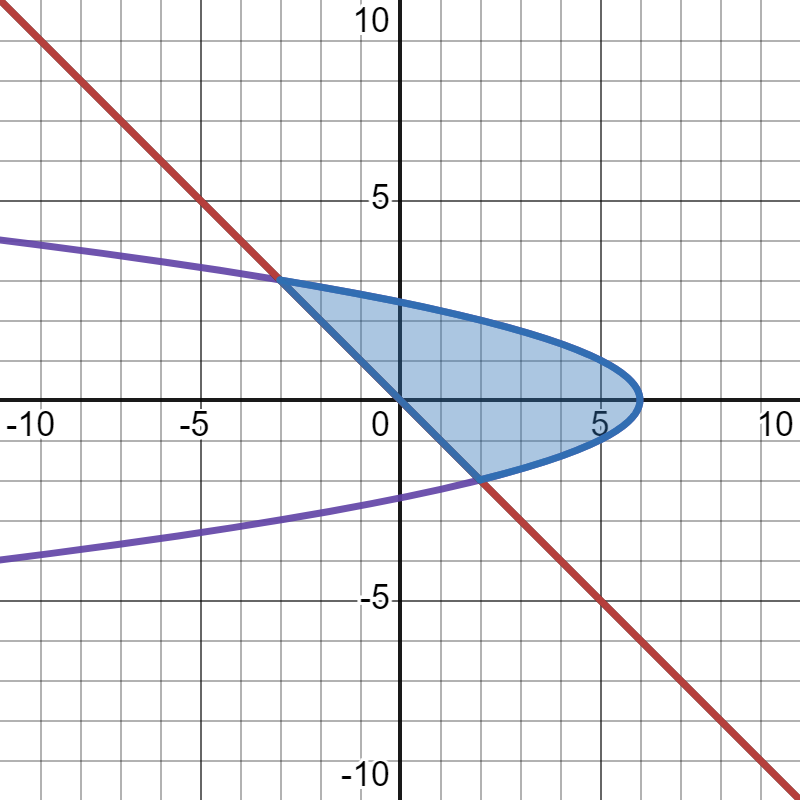
\includegraphics[width=150px]{15-2-1.png}

\newpage\subsubsection{Example 2}
Evaluate $\int\Int{D}{}(x+y)dA$ where $D$ is the region bounded by $y=\sqrt{x}$ and $y=x^2$
\paragraph{Solution}
$\int\Int{D}{}(x+y)dA=\Int{0}{1}\Int{x^2}{\sqrt{x}}(x+y)dydx$
\\$=\Int{0}{1}xy+\frac{y^2}{2}\eval{y=x^2}{\sqrt{x}}dx$
\\$=\Int{0}{1}\left(x\sqrt{x}+\frac{\sqrt{x}^2}{2}\right)-\left(xx^2+\frac{(x^2)^2}{2}\right)dx
\\=\Int{0}{1}\left(x^{\frac{3}{2}}+\frac{x}{2}-x^3-\frac{x^4}{2}\right)dx$
\\$=\frac{x^{\frac{5}{2}}}{\frac{5}{2}}+\frac{x^2}{4}-\frac{x^4}{4}-\frac{x^5}{2(5)}\eval{0}{1}$
\\$=\frac{2}{5}+\frac{1}{4}-\frac{1}{4}-\frac{1}{10}=\frac{4-1}{10}=\frac{3}{10}$

\subsubsection{Example 3}
Evaluate $\int\Int{D}{}2xydA$, where $D$ is the triangular region with vertices $(0,0)$, $(1,2)$ and $(0,3)$.
\paragraph{Solution}
Use the equation $m=\frac{y_2-y_1}{x_2-x_1}$ for the points $(0,0)$ and $(1,2)$ to get $y-y_1=m(x-x_1)$
to get $y=2x$, then do the same with $(0,3)$ and $(1,2)$ to get the equation $y=-x+3$
\\We then get: $\int\Int{D}{}2xydA=\Int{0}{1}\Int{2x}{-x+3}2xydydx$
\\$=\Int{0}{1}2x\frac{y^2}{2}\eval{2x}{-x+3}dx
\\=\Int{0}{1}\left[x(-x+3)^2-x(2x)^2\right]dx
\\=\Int{0}{1}\left[x(x^2-6x+9)-x(4x^2)\right]dx
\\=\Int{0}{1}(x^3-6x^2+9x-4x^3)dx
\\=\Int{0}{1}(-3x^3-6x^2+9x)dx
\\=\frac{-3x^4}{4}-\frac{6x^3}{3}+\frac{9x^2}{2}\eval{0}{1}
\\=\left(\frac{-3}{x}-2+\frac{9}{2}\right)-(0)
\\=\frac{-3-8+18}{4}=\frac{7}{4}$

\subsubsection{Example 4}
Evaluate $\Int{0}{1}\Int{x^2}{1}x^3\sin(y^3)dydx$
\paragraph{Solution}
We cannot integrate $\int sin y^3dy$. Therefore, we must reverse the order of integration.
\\$\Int{0}{1}\Int{x^2\to y=x^2}{1\to y=1}x^3\sin(y^3)dydx=\Int{0}{1}\Int{0}{\sqrt{y}}x^3\sin(y^3)dxdy$
\\$=\Int{0}{1}\frac{x^4}{4}\sin(y^3)\eval{0}{\sqrt{y}}dy=\Int{0}{1}\frac{(\sqrt{y})^4}{4}\sin(y^3)-0dy$
\\$=\Int{0}{1}\frac{y^2}{4}\sin(y^3)dy$, let $u=y^3$, $du=3y^2dy$
\\$=\int\frac{1}{4}\sin udu=\frac{-1}{12}\cos(y^3)\eval{0}{1}=\frac{-1}{12}(\cos1-\cos0)=\frac{-1}{12}(\cos1-1)$

\subsection{Applications of Double Integral}
\textbf{Area} $=\int\Int{D}{}dA$
\\\textbf{Volume} $=\int\Int{D}(z_{upper}-z_{lower})dA$
\newpage\subsubsection{Example 5}
Use double integrals to compute the area of the region bounded by $y=x^2$ and $y=2-x$
\paragraph{Solution} Calculate the POIs of the equations: $x^2=2-x\Rightarrow x^2+x-2=0\Rightarrow (x+2)(x-1)=0\Rightarrow x=-2,1$
\\Now, Area $=\Int{-2}{1}\Int{x^2}{2-x}dydx=\Int{-2}{1}y\eval{x^2}{2-x}dx$
\\$=\Int{-2}{1}(2-x-x^2)dx=2x-\frac{x^2}{2}-\frac{x^3}{3}\eval{-2}{1}$
\\$=(2-\frac{1}{2}-\frac{1}{3})-(2(-2)-\frac{(-2)^2}{2}-\frac{(-2)^3}{3})=\frac{7}{6}-\frac{-10}{3}=\frac{7+20}{6}=\frac{9}{2}$

\subsection{Midterm on July 4th, CHN G133}
Covers sections 12.5, 12.6, 13.1-13.4, 14.1-14.8
\begin{itemize}
    \itemsep 0em
    \item Sction 12.5 (1 or 2 questions): \begin{itemize}
        \itemsep 0em
        \item Equation of a line: $\vec{r}=\vec{r_0}+t\vec{v}$, in the case of tangent line: $\vec{V}=\vec{r}(t_0)$ where $\vec{V}$ is the direction vector.
        \item Equation of a plane: $a(x-x_0)+b(y-y_0)+c(z-z_0)=0$, in the case of a tangent plane: $\vec{n}=\tri f$ (sections 14.4 and 14.6)
    \end{itemize}
    \item Section 13.1 (2 or 3 questions): \begin{itemize}
        \itemsep 0em
        \item 13.1: Domain $\vec{r}(t)=<f(t),g(t),h(t)>$ and limits $\lim \vec{r}(t)=<\lim f,\lim g,\lim h>$
        \item 13.2: Derivatives $\vec{r}'(t)=<f'(t),g'(t),h'(t)>$ and integrals $\int\vec{r}(t)dt=<\int fdt,\int gdt,\int hdt>$ (covered indirectly).
        \item Unit tangent vector $\vec{T}(t)=\frac{\vec{r}'(t)}{|\vec{r}'(t)|}$ and unit normal vector $\vec{N}=\frac{\vec{T}'(t)}{|\vec{T}'(t)|}$
    \end{itemize}
    \item Section 13.3 (1 question): Arc length $=\Int{a}{b}|\vec{r}'(t)|dt$
    \item 1 question: Curvature $K=\frac{|\vec{T}'(t)|}{|\vec{r}'(t)|}$ or $K=\frac{|\vec{r}'\times\vec{r}''|}{|\vec{r}'|^3}$
    \item Chapter 3 (section 14.2) (4,5 or 6 questions): limits and continuity: \begin{itemize}
        \itemsep 0em
        \item Sub in $x=a$ and if we get an answer, we get the limit.
        \item If it is $\frac{0}{0}$, then we need to do any of the following: factorization, rationalization, polar coordinates, etc.
        \item We can show two paths with different answers to show that the limit does not exist.
        \item L'Hopital's rule only works with one variable.
        \item You can use polar coordinates to potentially show if the limit depends on $\theta$, then the limit DNE.
    \end{itemize}
    \item Section 14.7: local maximum/minimum, saddle point: \begin{itemize}
        \itemsep 0em
        \item If $f_x=0$ and $f_y=0$, then you have a critical point.
        \item $D=\mat{f_{xx}}{f_{xy}}{f_{xy}}{f_{yy}}$. If $D<0\Rightarrow$ saddle point, otherwise it is a local minimm or maximum.
        \item If $D>0$ and $f_{xx}>0$, then it is a local minimum. If $f_{xx}<0$ then it is a local maximum.
    \end{itemize}
    \item Optimization problem (1 question): \begin{itemize}
        \itemsep 0em
        \item You can eliminate $z$ and use section 14.7.
        \item If not, use Lagrange multipliers: find the maximum or minimum values of $f(x\dots)=\dots$ subject to $dots$.
    \end{itemize}
    \item Section 12.6: Quadric surfaces (no direct questions).
    \item Section 14.3: partial derivatives (covered indirectly).
    \item Section 14.4: tangent plane and linear approximation: $f(x,y)\approx f(a,b)+f_x(a,b)(x-a)+f_y(a,b)(y-b)$
    \item Section 14.6: directional derivative: $D_uf=\tri f\cdot\vec{u}$ where $\vec{u}$ is the unit vector.
\end{itemize}

\end{document}